\section{Resultados y Conclusiones}
% Deben incluir los resultados de los experimentos, utilizando el formato mas
% adecuado para su presentacion. Deberan especicar claramente a que
% experiencia corresponde cada resultado. No se incluiran aqu corridas de
% maquina. Algo fundamental en su aprendizaje en la materia es la presentacion
% de resultados de forma clara y concisa para el lector

% Se incluira aqu un analisis de los resultados obtenidos en la seccion
% anterior (se analizara su validez, coherencia, etc.). Deben analizarse como
% materianimo los lostems pedidos en el enunciado. No es aceptable decir que
% \los resultados fueron los esperados", sin hacer clara referencia a la
% teoremasa a la cual se ajustan. Ademas, se deben mencionar los resul- tados
% interesantes y los casos \patologicos" encontrados.

\subsection{Hipótesis}
Como vimos en la Introducción Teórica, Newton tiene convergencia cuadrática y
Secante $supralineal$ (alrededor de 1.6).

Sería normal suponer que Newton tiene mejor performance dado que converge más
rápido. Sin embargo para comparar performance, debemos considerar costo como
rapidez de convergencia. Un algoritmo que converge rápido pero tarda algunos
segundos por iteración podría tomar mas tiempo que uno que converge mas lento
pero toma solo algunos milisegundos por iteración.

Podemos asumir que el costo de una iteración está marcado por la evaluación de
la función, de hecho, este vendría a ser nuestro caso. Entonces la cantidad de
evaluaciones de una función puede ser una buena medida de costo.

Secante solo requiere una evaluación de la función por iteración, dado que el
valor de $f(x_{n - 1})$ se puede guardar de la iteración previa.

Newton requiere una evaluación de la función y otra de su derivada por
iteración. Es complicado estimar el costo de evaluar la derivada en general. En
algunos casos la derivada puede ser fácil de evaluar y en otros puede ser
incluso mas difícil de evaluar que la función original.

Podemos asumir entonces, que en general, calcular la derivada es al menos tan
costoso como calcular la función. Por lo tanto asumimos que Newton va a tomar
dos evaluaciones por iteración.

Este análisis nos lleva a suponer que Secante debería ser mas performante que
Newton en general.

\subsection{Casos de Prueba}
La aproximación inicial que tuvimos fue tomar cada uno de los parámetros, fijar
los demás y hacer un análisis de cada uno de los factores de estudio (tiempo,
iteraciones, convergencia, etc.) haciendo crecer los parámetros de turno.
Claramente la cantidad de casos era mucha y en general los resultados eran
difíciles de interpretar y no aportaban al propósito de develar si nuestra
hipótesis se cumplía.

Por lo tanto decidimos que lo mejor sería solamente tomar un par de
combinaciones de todas las posibles que nos parecieran que fueran
representativas. En nuestro caso al ya tener $x_0$ y $x_1$ definidos en base a
previa experimentación decidimos hacer comparaciones entre los métodos en
términos de iteraciones y tiempo de ejecución para $\alpha$'s crecientes.

\subsubsection{Iteraciones} % (fold)
\label{ssub:iteraciones}

En el caso de hacer crecer $\alpha$ para ver cómo se comportan en función de
las iteraciones, nuestra suposición es que Newton tomará menos iteraciones que
Secante. Ahora, para Newton con $f(x)$ y $e(x)$ suponemos que el primero tomará
menos iteraciones ya que el segundo cuenta con un cociente extra para calcular
con respecto al primero en cada iteración.

\begin{figure}[!htbp]
  \begin{center}
    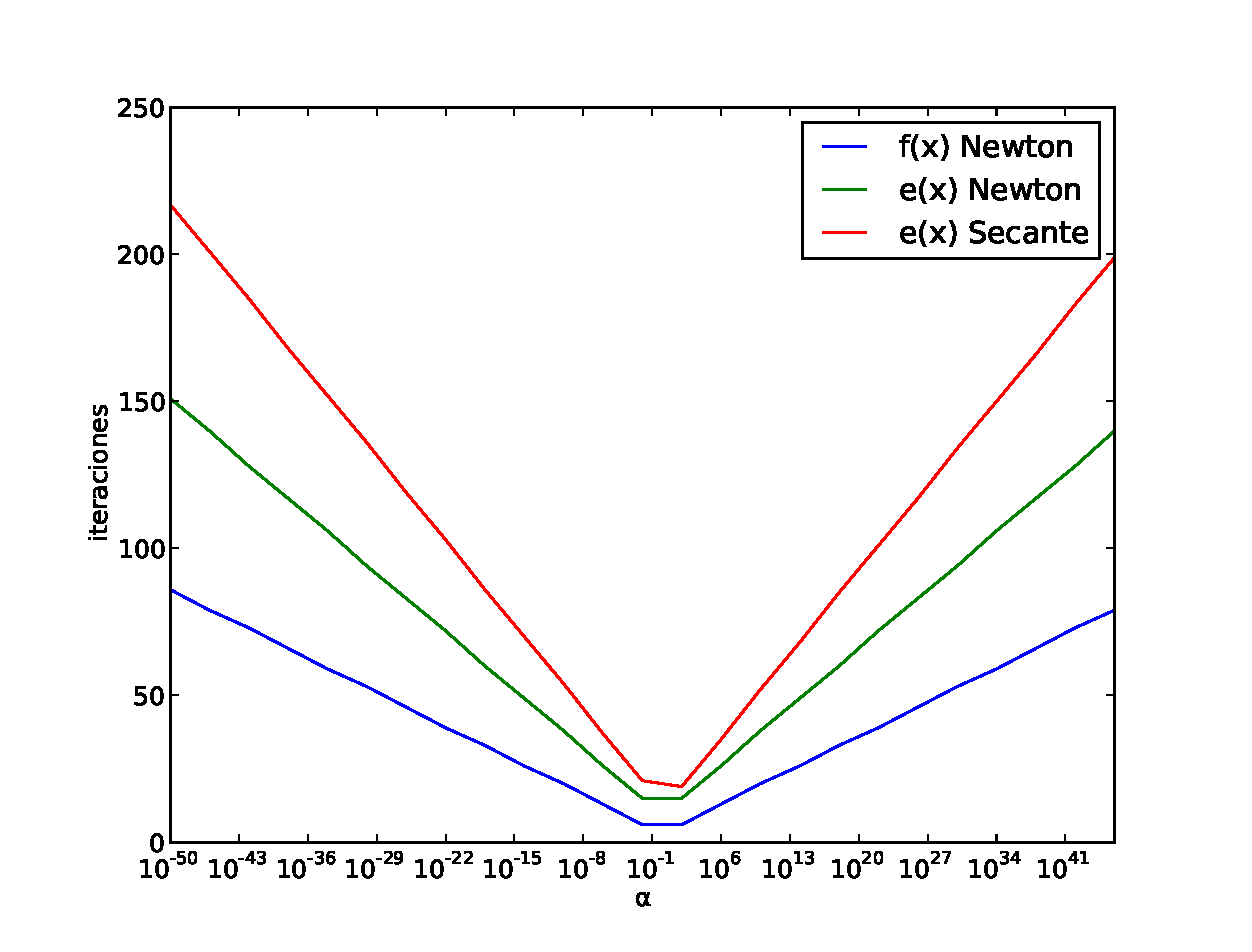
\includegraphics[scale=0.5]{graficos/new/comparacion_iteraciones.eps}
    \caption{\label{fig:comparacion_iteraciones} Gráfico comparativo de $\alpha$ en función de la cantidad de iteraciones}
  \end{center}
\end{figure}

Como podemos ver en la Figura~\ref{fig:comparacion_iteraciones} nuestras
expectactivas se cumplieron, y podemos ver además como las iteraciones
disminuyen a medida que los puntos iniciales están cerca del $\alpha$.

% subsubsection iteraciones (end)

\subsubsection{Tiempo de Ejecución} % (fold)
\label{ssub:tiempo_de_ejecuci_n}

Para hacer el cálculo del tiempo lo que hicimos fue hacer 1000 corridas de cada
método y luego tomar el promedio, de esta manera podemos descartar outliers. En
esta sección entra en juego lo que mencionamos en la parte de Hipótesis. En
términos prácticos, uno de los factores a tomar en cuenta es cuán rápido
obtenemos el resultado requerido. Como bien enunciamos anteriormente, suponemos
que Secante será mas rápido que Newton.

\begin{figure}[!htbp]
  \begin{center}
    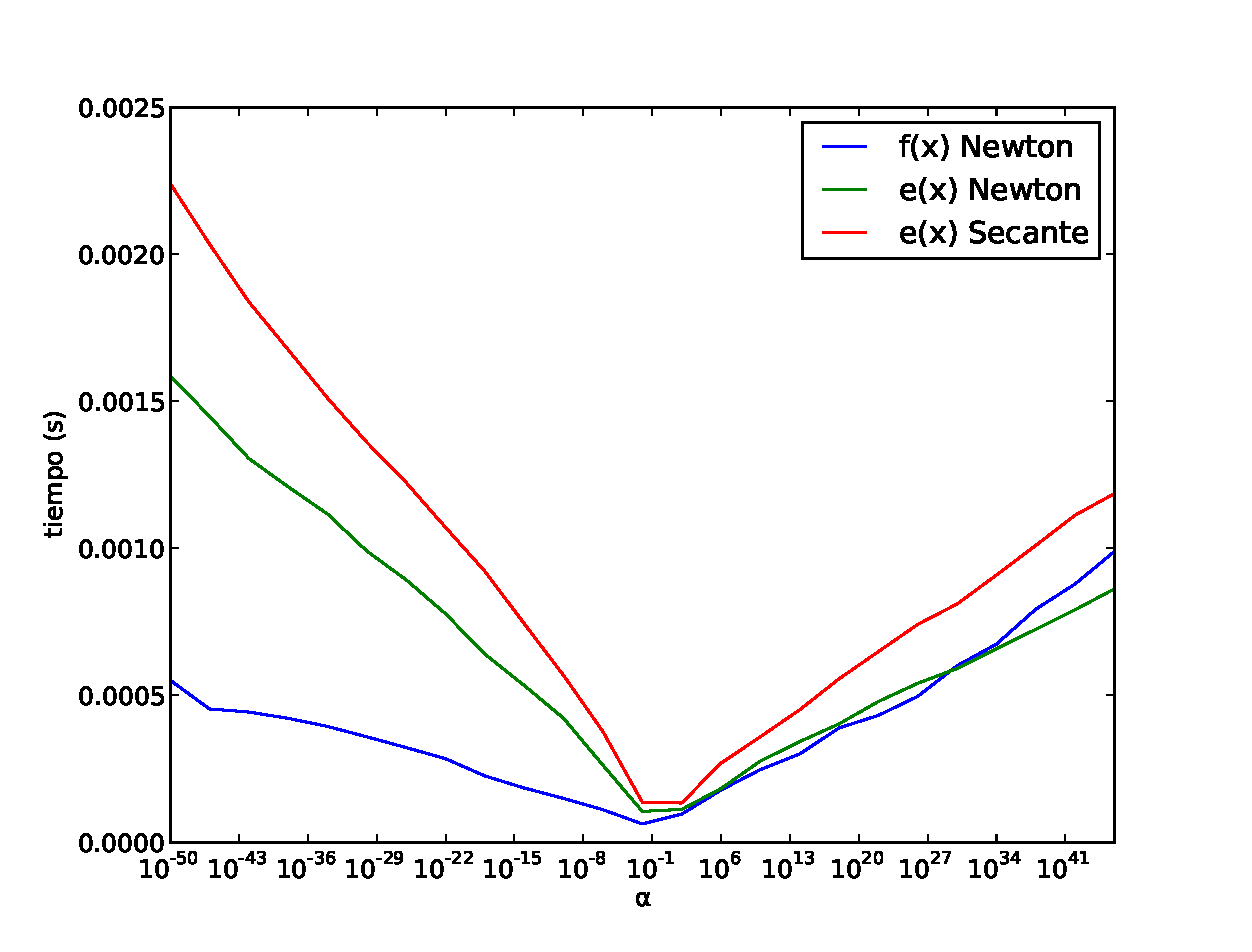
\includegraphics[scale=0.5]{graficos/new/comparacion_tiempos.eps}
    \caption{\label{fig:comparacion_tiempos} Gráfico comparativo de $\alpha$ en función del tiempo de ejecución}
  \end{center}
\end{figure}

En la Figura~\ref{fig:comparacion_tiempos} vemos cómo lo que habíamos
anticipado al final no sucede, Newton con $f(x)$ es el que termina siendo mas
performante y lo otro que podemos ver es que para $e(x)$ con Newton y Secante,
el primero es mas performante desde valores chicos, pasando por el valor
exacto, hasta que cuando $alpha$ crece mas, llega un punto donde Newton supera
a Secante.

% subsubsection tiempo_de_ejecuci_n (end)
\section{Discusión y Conclusiones}

En esta parte analizaremos, cuestionaremos y concluiremos sobre aquellos puntos
que nos parecieron interesantes pero que además fueron preponderantes en el
desarrollo del presente trabajo.

\subsection{Elección de los puntos iniciales de las sucesiones} % (fold)
\label{sub:elecci_n_de_los_puntos_iniciales_de_las_sucesiones}

En la secciones \ref{ssub:ajuste_f_x0_newton}, \ref{ssub:ajuste_e_x0_newton}, \ref{ssub:ajuste_e_x0_x1_secante}
% Hablar sobre las variantes que descartamos al hacer este tipo de enfoque y sus posibles repercusiones

% subsection elecci_n_de_los_puntos_iniciales_de_las_sucesiones (end)

\subsection{Análisis de los resultados en función del tiempo y las iteraciones} % (fold)
\label{sub:an_lisis_de_los_resultados_en_funci_n_del_tiempo_y_las_iteraciones}

\subsubsection{Iteraciones} % (fold)
\label{ssub:iteraciones}

Para este gráfico (Figura~\ref{fig:comparacion_iteraciones}) no existe
demasiada discusión ya que el resultado cumple con las expectativas que
teníamos previamente. Cabe destacar que las pendientes de las rectas con
respecto al origen en módulo no son iguales, esto es interesante dado que el
análisis previo de cada función nos mostró que podíamos hacer uso indistinto de
cualquiera de las raíces, lo cual hacía suponer que el gráfico tendría que
tener mayor simetría.

Mas allá de estos detalles, pudimos cerciorar empíricamente que si se toma en
cuenta la cantidad de iteraciones, usando $f(x)$ con el método de Newton es la
opción mas recomendable

% subsubsection iteraciones (end)

\subsubsection{Tiempo de ejecución} % (fold)
\label{ssub:tiempo_de_ejecuci_n}

En esta gráfico (Figura~\ref{fig:comparacion_tiempos}) es en donde pudimos ver
un comportamiento al menos no esperado de nuestra parte. Suponemos que nuestra
hipótesis no se cumple, pues la derivada en este caso es fácil de calcular y
evaluar, haciendo que el factor que menos beneficiaba a este método no afecte
para este caso a la performance.

% subsubsection tiempo_de_ejecuci_n (end)

% subsection an_lisis_de_los_resultados_en_funci_n_del_tiempo_y_las_iteraciones (end)

\subsection{Resoluciones finales} % (fold)
\label{sub:resoluciones_finales}

% subsection resoluciones_finales (end)

\subsection{Trabajos futuros} % (fold)
\label{sub:trabajos_futuros}

% subsection trabajos_futuros (end)
